\documentclass{SPhdThesis}

% PDF and title properties.
\SgSetTitle{FOC Firmware for Integrated BLDC Driver}
\SgSetAuthor{Mathias Palme}
\SgSetYear{2026}
\SgSetSupervisor{Ing. Krištof Pučejdl}
\SgSetDegree{Bachelor's thesis}
\SgSetUniversity{Czech Technical University in Prague}
\SgSetFaculty{Faculty of Electrical Engineering}
\SgSetDepartment{Department of Control Engineering}	
\SgSetDeclarationDate{May 2026}

% Make the nomenclature
\usepackage{nomencl}
\makenomenclature

% Command for TODO things
\newcommand\todo[1]{\textcolor{red}{#1}}


\makenomenclature
\setlength{\nomlabelwidth}{3cm}
\setlength{\nomitemsep}{-\parsep}

% The document.
\begin{document}
	\begin{frontmatter}
		% Cover is not done yet
		%\coverimage{}
		%\makecover
		\SgAddTitle{ctu_logo/cvut_symbol.pdf}%
		\ctuAddAssignment{pdf_input_files/assignment.pdf}%
		\SgAddDeclaration%
		\begin{acknowledgments}
Acknowledgment section need not to be too strict. Try to express your personality, sense of humor and so on :). 



\end{acknowledgments}
%
		\begin{abstract}
{
The goal of this thesis is developing and testing embedded software that implements Field Oriented Control
(FOC) for Brushless DC (BLDC) motors on an existing integrated three-phase motor driver called uFOC (micro FOC) with an STM-32
type microcontroller developed by Bc. Šimon Pecháček and Ing. Krištof Pučejdl at the Department of Control Engineering, Faculty of Electrical Engineering, Czech Technical University in Prague.
The firmware implements FOC control algorithm to control torque. On top of torque control a PI velocity and PID position control loop is implemented. 
Aditionally communication via CAN bus is implemented with daisy chaining of multiple drivers, to allow indepemendent control and sensor readings from each driver via a signle CAN bus line.
\\
\\
\textbf{Keywords:} FOC, BLDC, embedded software, motor control.
}

% ------------- 

{
Česká verze abstraktu (anotace) s klíčovými slovy na konci.
Doplnit českou verzi...
\\
\\
\textbf{Klíčová slova:} antikolizní systém, digitální mapa, kalmanův filtr, V2X-komunikace.
}
\end{abstract}%
		
		\SgAddToc%  Table of contents.
		% ---------------		
		% In my opinion, LoF, LoT or LoA are useless in the thesis.
		% ---------------
		%\SgAddLof%  List of figures.
		%\SgAddLot%  List of tables.
		%\SgAddLoa%  List of algorithms.
		\nomenclature[A]{CAM}		{Cooperative awareness message.}
\nomenclature[A]{CAN}		{Controller Area Network (bus).}
\nomenclature[A]{DEM}		{Digital elevation model.}
\nomenclature[A]{DOF}		{Degree of freedom.}

\nomenclature[N]{$x_{c,k}$}						{Clearance at time $k$.}
\nomenclature[N]{$x_{k}$}						{State vector at time $k$.}
\nomenclature[N]{$y_{k}$}						{Measurement vector at time $k$.}

\nomenclature[M]{$A^\intercal$}					{Transposition of a matrix $A$.}
\nomenclature[M]{$D$}							{Time delay.}
\nomenclature[M]{$F_k$}							{System (state) matrix of the system in time $k$.}

\nomenclature[G]{$\Delta t$}						{Sampling period of the system.}
\nomenclature[G]{$\psi, \theta, \phi$}				{Heading, slope and bank angles.}
\nomenclature[G]{$\omega_x,\omega_y,\omega_z$}		{Measured angular rate around an axis $x,y,z$.}

\nomenclature[O]{$\approx$}							{Approximation.}
\nomenclature[O]{$\coloneqq$}						{Assignment.}
\nomenclature[O]{$\triangleq$}						{Definition.}
	
		\printnomenclature
	\end{frontmatter}
	
	% Divide document into several parts
	\chapter{Introduction}
BLDC and PMSM motors are increasingly more popular in varous applications, such as robotics, drones, electric vehicles and many more, due to their high efficiency, 
ability to produce large torque at low speeds and high position accuracy. Unlike brushed DC or universal motors, 
BLDC motors need specialized driver and control to achieve commutation.

While commercial BLDC drivers are available on todays market, such as ODrive Micro, moteus-c1, 
they are often expensive in range of 70-90 USD per driver. \cite{moteus_c1} \cite{odrive_micro}
Therefore, the Department of Control Engineering at the Czech Technical University in Prague has developed an 
integrated three-phase motor driver called uFOC (micro FOC) with an STM-32 type microcontroller, 
which is a low-cost alternative to commercial drivers at BOM price of approximately 20 USD. \cite{uFOC}

The goal of the uFOC project was to develop a compact integrated motor driver for dynamic servo actuators, 
containing all components required for closed-loop torque control on a single printed circuit board.
The concept of tightly integrating the motor, driver electronics, 
and communication interfaces into a compact actuator unit was inspired by the modular actuator design presented
by Benjamin Katz in his work on low-cost actuators for dynamic robots. \cite{ben_katz}
The current revision of the uFOC driver has dimensions of 30×30~mm, approaching the practical physical limits imposed by components such as connectors.
The driver is intended for direct mounting onto the motor assembly, minimizing external wiring requirements to only power and CAN bus connections.
Two CAN connectors are provided to support daisy-chain communication in multi-actuator systems. \cite{uFOC}

To achive an efficient commutation and generate torque, the driver needs to implement a closed loop control.
The most common control method for BLDC motors is Field Oriented Control (FOC), 
which allows for precise control of the motor's torque, speed and position by controlling the current in the stator windings.

Goal of this thesis is to develop embedded firmware that implements FOC current control, speed and position control loops and communication via CAN bus for the uFOC driver. 
Additionally a Python client side example for CAN communication with the driver is provided.



	\chapter{Brief explanation of FOC}
\section{FOC overview}
Field Oriented Control (FOC) is a closed loop control method for controlling torque of BLDC motors based on Clarke-Park Transformation.
Standard BLDC motor is aquipped with three stator windings, which are supplied with three phase currents.
To achive commutation and generate torque, propper voltage has to be provided to the stator windings by reading the phase currents ($i_a, i_b, i_c$).
Three phase currents reference frames can be decomposed into two orthogonal torque and flux reference frames using Clarke transformation, 
resulting in two currents ($i_\alpha$, $i_\beta$) in a stationary reference frame.

Park transformation is then applied to transform the currents from a stationary reference frame to a rotating reference frame, resulting in two DC currents ($i_d$, $i_q$), 
where $i_d$ is a flux current and $i_q$ is a torque current.

To control $i_d$ and $i_q$ currents, two independent proportional-integral (PI) controllers are used to update applied voltage to the stator windings based on the error between the reference and the measured currents.
In this implementation only the $i_q$ current reference is changed to control the torque, while the $i_d$ current reference is always set to zero to maximize the torque per ampere.

After getting new voltage references from the PI controllers, they need to be transformed back to three phase voltages using inverse Park and inverse Clarke transformations,
which can be then applied to the stator windings.

However applying the voltages directly from the inverse Park-Clarke transformations will achieve only aproximatelly 85 \% of the maximum voltage difference between the stator windings,
which is not optimal. \cite{svpwm_efficiency} To maximize the voltage difference between the stator windings, Space Vector Modulation (SVPWM) can be applied to the voltage references. 

Now that we can control the torque of the motor by controlling the $i_q$ current reference, a velocity control loop can be implemented on top of the torque control by 
using a PI controller to update the $i_q$ current reference based on the velocity error.

Aditionally, a position control loop can be implemented on top of the velocity control loop by using a PID controller to update the velocity reference based on the position error.

\begin{figure}[h]
    \centering
    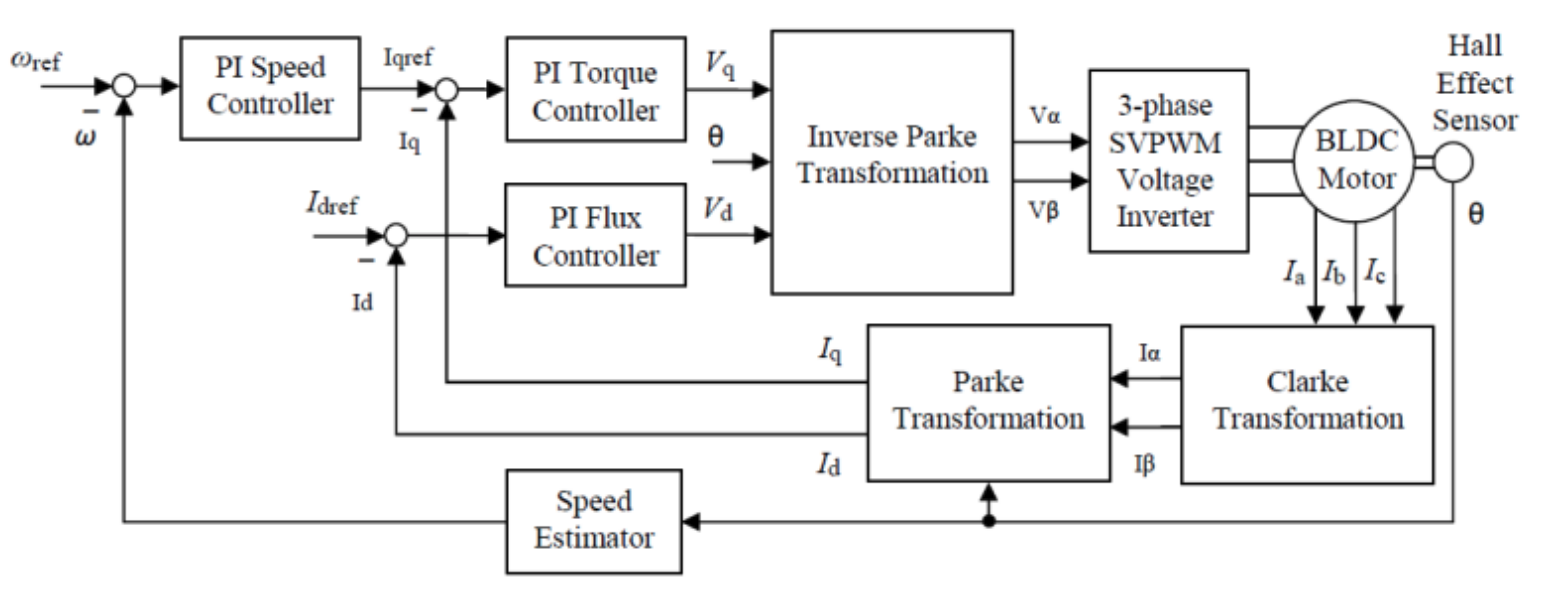
\includegraphics[width=0.95\textwidth]{figs/foc_diagram.png}
    \caption{Field Oriented Control block diagram. \cite{block_diagram_foc}}
    \label{fig:foc_diagram}
\end{figure}

The Figure~\ref{fig:foc_diagram} shows the cascaded structure of the FOC control system. 



\section{Clarke transformation}
Clarke transformation is used to transform three phase currents ($i_a$, $i_b$, $i_c$) into two orthogonal currents ($i_\alpha$, $i_\beta$) in a stationary reference frame,
where $i_\alpha$ is torque generating current and $i_\beta$ is flux producing current.

Clarke transformation can be represented as a matrix multiplication of the three phase currents with the transformation matrix
\begin{equation}
\begin{bmatrix}
i_\alpha \\
i_\beta
\end{bmatrix}
=
\frac{2}{3}
\begin{bmatrix}
1 & -\frac{1}{2} & -\frac{1}{2} \\
0 & \frac{\sqrt{3}}{2} & -\frac{\sqrt{3}}{2}
\end{bmatrix}
\begin{bmatrix}
i_a \\
i_b \\
i_c
\end{bmatrix}.
\end{equation}

The scaling factor $\frac{2}{3}$ ensures amplitude invariance between the three-phase and $i_\alpha$ $i_\beta$ representations.

The Figure~\ref{fig:clarke_transformation} shows a Clarke transformation of 3-phase sinusoidal current into two orhogonal currents. 

\begin{figure}[h]
    \centering
    \includegraphics[width=0.95\textwidth]{figs/clarke_transformation.pdf}
    \caption{Clarke transformation of three-phase current.}
    \label{fig:clarke_transformation}.
\end{figure}

% The Figure~\ref{fig:clarke_transformation} shows a Clarke transformation of 3-phase sinusoidal current. 


Inverse Clarke transformation in context of FOC is used to transform two orthogonal voltages ($v_\alpha$, $v_\beta$) in a stationary reference frame back
to three phase voltages ($v_a$, $v_b$, $v_c$) that can be applied to the stator windings and can be expressed as
\begin{equation}
\begin{bmatrix}
v_a \\
v_b \\
v_c
\end{bmatrix}
=
\begin{bmatrix}
1 & 0 \\
-\frac{1}{2} & \frac{\sqrt{3}}{2} \\
-\frac{1}{2} & -\frac{\sqrt{3}}{2}
\end{bmatrix}
\begin{bmatrix}
v_\alpha \\
v_\beta
\end{bmatrix}.
\end{equation}





\section{Park transformation}
Park transformation is used to transform two orthogonal currents ($i_\alpha$, $i_\beta$) in a stationary reference frame from the stator point of view
into two DC currents ($i_d$, $i_q$) in a rotating reference frame from a rotor point of view, where $i_d$ is a flux current and $i_q$ is a torque current.
To perfrom Park transformation, the electrical angle $\theta_e$ must to be calculated based on the rotor position, which can be obtained from the encoder reading.

Park transformation can be represented as a matrix multiplication of the two orthogonal currents ($i_\alpha$, $i_\beta$) with the transformation matrix

\begin{equation}
\begin{bmatrix}
    i_d \\
    i_q
\end{bmatrix}
=
\begin{bmatrix}
\cos(\theta_e) & \sin(\theta_e) \\
\sin(-\theta_e) & \cos(\theta_e)
\end{bmatrix}
\begin{bmatrix}
    i_\alpha \\
    i_\beta
\end{bmatrix} .
\end{equation}


Figure~\ref{fig:park_transformation} shows the Park transformation applied to the output of the 
Clarke transformation shown in Figure~\ref{fig:clarke_transformation}, resulting in two DC current components.

\begin{figure}[h]
    \centering
    \includegraphics[width=0.95\textwidth]{figs/park_transformation.pdf}
    \caption{Park transformation of Clarke transformation output}
    \label{fig:park_transformation}
\end{figure}

% The Figure~\ref{fig:park_transformation} shows Park transformation of the previous output of Clarke transformation from Figure~\ref{fig:clarke_transformation}.




In context of FOC, inverse Park transformation is used to transform two orthogonal DC voltages ($v_d$, $v_q$), which are the outputs of the PI controllers, 
from a rotating reference frame back to two orthogonal voltages ($v_\alpha$, $v_\beta$) in a stationary reference frame.

Inverse park transformation can be represented as a matrix multiplication of the two orthogonal DC voltages ($v_d$, $v_q$) with the transformation matrix
\begin{equation}
\begin{bmatrix}
v_\alpha \\
v_\beta
\end{bmatrix}
=
\begin{bmatrix}\cos(\theta_e) & -\sin(\theta_e) \\
\sin(\theta_e) & \cos(\theta_e)
\end{bmatrix}
\begin{bmatrix}v_d \\
v_q
\end{bmatrix}.
\end{equation}

\section{PI and PID regulators}

Proportional-Integral (PI) controllers are used in the FOC algorithm to regulate the $d$-axis and $q$-axis currents by adjusting the corresponding voltages ($v_d$, $v_q$).
To prevent integrator windup during saturation conditions, anti-windup protection is implemented by limiting the integration process. 
The discrete-time PI controller with anti-windup can be expressed as

\begin{equation}
x_{out}(k+1) =
K_p x_{in}(k)
+
w_{up} K_i T_s x_{in}(k)
+
x_{out}(k),
\end{equation}

where

\begin{equation}
w_{up} =
\begin{cases}
1, & \text{if } -x_{lim} < x_{in}(k) < x_{lim} \\
0, & \text{otherwise}
\end{cases}
\end{equation}

and $x_{lim}$ is the integral component limit. \cite{prayogo_foc}

The proportional term provides immediate response to the control error, while the integral term eliminates steady-state error.
In the implemented cascaded control structure, PI controllers are used for current and velocity regulation.

For position control, a Proportional-Integral-Derivative (PID) controller is additionally used to improve damping and reduce overshoot.
The PID controller generates the target angular velocity for the inner velocity control loop. \cite{SimpleFOC}


\section{Space vector modulation}

Space Vector Pulse Width Modulation (SVPWM) is used to efficiently generate three-phase PWM signals for the inverter from the calculated voltage references.
Compared to sinusoidal PWM, SVPWM provides better utilization of the DC bus voltage and allows approximately 15~\% higher maximum output voltage. \cite{svpwm_efficiency}
After inverse Park and inverse Clarke transformations generate the three-phase voltage references ($v_a$, $v_b$, $v_c$),
SVPWM computes the duty cycles for individual inverter phases and applies them to the MOSFET bridge.

The simplified SVPWM duty cycle equation can be expressed as

\begin{equation}
d_i = 0.5V_{dc} + v_{ref_i} + U^{*},
\end{equation}

where

\begin{equation}
U^{*} = -0.5 \left( \max\left(\sum_i v_{ref_i}\right) + \min\left(\sum_i v_{ref_i}\right) \right),
\end{equation}

and $v_{ref_i}$ represents the phase voltage references for phases $a$, $b$, and $c$. \cite{prayogo_foc}

\section{Velocity and position control loops}

The FOC torque control loop directly regulates the motor torque through the $i_q$ current component.
Once torque control is established, higher-level control loops can be added on top of the inner current loop in order to control additional mechanical quantities.

Angular velocity control can implemented using a cascaded control structure. \cite{SimpleFOC}
The measured motor velocity derived from encoder readings is compared with the target velocity, 
and the resulting error is processed by a PI controller.
The output of the velocity controller generates the target torque-producing current $i_q$ for the inner FOC current control loop.
In this way, motor velocity is indirectly controlled through regulation of the generated motor torque.

Similarly, position control can be implemented as an additional outer control loop.
The measured rotor position is compared with the target position, and the resulting position error is processed by a PID controller.
The output of the position controller generates the target angular velocity for the velocity control loop.

This creates a cascaded control hierarchy consisting of:
\begin{itemize}
    \item current control loop regulating motor torque,
    \item velocity control loop regulating angular velocity,
    \item position control loop regulating rotor position.
\end{itemize}

The cascaded structure allows simultaneous control of motor torque, angular velocity, and position while maintaining stable dynamic behaviour.
Typically, the inner current loop operates at the highest update frequency, while the outer velocity and position loops operate at lower frequencies
due to slower mechanical system dynamics.

\section{Electrical angle calculation}


	\chapter{Firmware implementation}
\section{Used technologies and development tools}
STM32CubeMX was used to simplify the initial project setup, while the HAL library was employed to facilitate peripheral configuration
and management. The firmware was implemented in the C programming language. CAN communication testing was performed using a 
Makerbase CANable V2.0 USB interface together with a Python based client script built on the pycan library. 
* Also compilation should be mantioned * 

Arduino IDE was used as a serial monitor for debugging purposes.
\section{Firmware topology}
The firmware is structured into reusable modules located in the \texttt{uFOC\_lib} directory. 
Peripheral initialization and high-level application logic are implemented in \texttt{src/main.c}.

uFOC\_lib contains the following modules:
\begin{itemize}
    \item \texttt{driver} - handles DRV8316CRRGFR driver configuration and control, ADC current sensing and PWM generation.
    \item \texttt{encoder} - handles MT6835GT encoder SPI configuration, positional data reading, 
                            angular velocity calculation and signal filtering.
    \item \texttt{foc} - implements all necessary transformations, to perform FOC control as well as 
                            trigonometric functions optimizations and SVPWM calculations.
    \item \texttt{config} - is used to store and control global configuration parameters of the firmware. 
                            This module implements an abstraction layer to simplify the access 
                            to the configuration parameters and ensure that they are updated correctly.
    \item \texttt{pi\_controller} - implements PI and PID controllers with anti-windup and output saturation.
    \item \texttt{communication} - manages CAN communication, including message parsing and sending.
\end{itemize}

The current control loop, together with current sampling and encoder reading, is executed in the ADC injected conversion complete interrupt,
which is triggered by the \texttt{TIM1\_CC4} event at a frequency of 8888~Hz. This ensures precise alignment between current measurement and the PWM cycle.
The selected control loop frequency corresponds to the maximum rate at which the current implementation of the FOC algorithm can be executed reliably.
The main performance limitation is currently the SPI based encoder communication.

Higher-level control loops, namely velocity and position control, are executed in a separate timer interrupt (\texttt{TIM6}) at a lower frequency of 2000~Hz, 
reflecting the cascaded structure of the control system.

This separation of control loops follows common practice in motor control systems, 
where fast inner loops regulate currents and slower outer loops regulate mechanical quantities.

\section{MCU configuration}

The uFOC driver uses an STM32F3xx microcontroller as the main processing unit. 
The MCU is responsible for real-time motor control, peripheral coordination, 
and communication with external devices. The configuration of the microcontroller is designed to 
meet the deterministic timing and low latency requirements of FOC.

\subsection{System clock}

The system clock is derived from the internal high-speed oscillator (HSI) operating at 8~MHz. 
This signal is multiplied using a phase-locked loop (PLL) with a multiplication factor of 16, resulting in a system clock frequency of 64~MHz.

The AHB bus runs at the full system clock frequency (64~MHz), while the APB1 bus is prescaled by a factor of 2 to 32~MHz, and the APB2 bus operates at 64~MHz. This configuration satisfies the peripheral frequency constraints while maintaining maximum performance for time-critical components.

Particular attention is given to peripherals involved in motor control. The advanced timer TIM1 and the ADC are both clocked at 64~MHz, ensuring high timing resolution for PWM generation and precise synchronization of current sampling.

This clock distribution enables deterministic timing of control loops and supports the strict real-time requirements of the control algorithm.

TIM6 is clocked from the APB1 timer clock. Although the APB1 peripheral clock is prescaled to 32~MHz, the timer clock is doubled to 64~MHz due to the APB1 prescaler being different from one. TIM6 is configured with a prescaler of 31 and an auto-reload value of 999, resulting in an update interrupt frequency of 2~kHz.


\subsection{Timer configuration}
The advanced timer TIM1 is used for PWM generation. It is configured in center aligned mode, 
which reduces switching harmonics and is commonly used in motor control applications. 
The timer operates at a PWM frequency of 8888~Hz. 

TIM1 also generates a compare event (\texttt{CC4}) that is used to trigger ADC injected conversions. 
This ensures that current sampling is synchronized with the PWM cycle and occurs at a well-defined point in time.

A separate basic timer, TIM6, is used to periodically execute higher-level control loops. 
TIM6 operates at a frequency of 2~kHz and triggers an interrupt used for velocity and position control. 
This lower update rate reflects the cascaded structure of the control system, 
where slower outer loops are executed less frequently than the inner current control loop.

\subsection{ADC configuration}
The ADC is configured to perform injected conversions of three phase currents.
The conversions are triggered by a TIM1 compare event, ensuring that current sampling occurs 
at a well-defined point within the PWM cycle. This synchronization minimizes measurement noise and improves control accuracy.

The ADC conversion complete interrupt is used to process the measured currents and execute the current control loop.

\subsection{PWM ADC synchronization}
In order to ensures deterministic timing and minimize control latency
a precise synchronization between PWM generation and current measurement is achieved by using a timer-generated trigger for ADC conversions.
The TIM1 compare event (\texttt{CC4}) initiates the ADC injected sequence, and the corresponding interrupt is used to execute the control algorithm.

The trigger signal is generated by a dedicated compare channel that is not used for PWM output, 
allowing independent adjustment of the sampling point within the PWM cycle.

\subsection{Communication interfaces}
The MCU communicates with external systems primarily via the CAN interface, which is used for command exchange and system control. 
The CAN peripheral is configured in normal mode with automatic retransmission enabled.

The CAN peripheral is clocked from the APB1 bus operating at 32~MHz. 
The bit timing parameters are configured to achieve a communication speed of 500~kbit/s. 
This interface is used for command exchange and system control and operates independently of the real-time control loops.

A UART interface is also available and is used only for debugging and diagnostic output during development.

SPI communication is used to interface with external peripherals, namely the magnetic encoder and the gate driver. 
Both devices share a single SPI peripheral, with separate chip-select signals used to access each device.

The SPI operates in master mode, and its configuration (clock polarity and phase) is adjusted as required by the connected peripherals.

The magnetic encoder is accessed within the real-time control loop to obtain rotor position information. 
The encoder update is performed inside the ADC interrupt service routine, 
ensuring that position data is synchronized with current measurements and control execution. 
As the SPI communication is performed in a blocking manner, its latency directly affects the execution time of the control loop.

In contrast, communication with the gate driver is primarily used for configuration. 
These operations are not time-critical and are performed outside the real-time control loop only during firmware initialization.

The SPI peripheral operates at a clock frequency of approximately 32~MHz, 
configured using a prescaler of 2. This high communication speed minimizes the duration of blocking SPI transactions, 
which is particularly important as encoder data acquisition is performed within the interrupt service routine.

% At this speed, the encoder read transaction takes only a few microseconds.

\section{Encoder}
The rotor position is measured using an MT6835 magnetic encoder with a 21-bit absolute resolution and SPI communication interface.\cite{datasheet_MT6835}
The encoder interface is implemented as a reusable module located in \texttt{uFOC\_lib/encoder}. This module provides encoder initialization, 
raw position acquisition, CRC verification, position unwrapping, velocity estimation, signal filtering and electrical offset calibration.

The encoder is accessed through the SPI3 peripheral. Since the SPI bus is shared with the gate driver, 
the encoder module explicitly configures the SPI peripheral before encoder communication. The encoder uses a dedicated chip-select signal, 
while the SPI transfer itself is performed in blocking mode. 
This is acceptable because the encoder read operation is executed inside the real-time control loop and must therefore be deterministic and short.

\subsection{Encoder data structure}

The encoder state is stored in the \texttt{encoder\_t} structure. It contains the most recent raw encoder value, the previous raw value, an unwrapped absolute position counter, velocity estimates, filtering parameters, electrical angle information and diagnostic variables related to CRC checking.

The raw encoder position is stored as a 21-bit value in the range from $0$ to $2^{21}-1$. To handle continuous rotation across the encoder overflow boundary, the module computes the difference between consecutive samples and corrects it when the difference exceeds half of the encoder range. The corrected difference is accumulated into \texttt{position\_ticks}, which represents the continuous mechanical position.

The structure also contains the \texttt{invert\_dir} flag. This flag allows the logical direction of rotation to be inverted without modifying the raw encoder data. It affects the sign of the computed mechanical position, angular velocity and electrical angle.

Namely \texttt{encoder\_t} contains:
\begin{itemize}
\item \verb|bool invert_dir| -- logical inversion of rotation direction which affects the sign of computed 
                                angle and velocity without modifying raw encoder data

\item \verb|uint32_t current_raw_value| -- latest 21-bit raw position value read from the encoder via SPI

\item \verb|uint32_t prevous_raw_value| -- previous raw position value, used to compute the delta between consecutive samples

\item \verb|float angular_velocity| -- instantaneous angular velocity estimate (in rotations per second), 
                                        computed from the filtered position increment

\item \verb|float angular_velocity_ewma| -- exponentially weighted moving average (EWMA) of angular velocity
                                            which is used for velocity control to reduce signal noise

\item \verb|float angular_velocity_ewma_alpha| -- EWMA coefficient $\alpha$ for velocity filtering,
                                                 defines the trade-off between responsiveness and noise suppression

\item \verb|float ewma_value| -- EWMA filtered absolute position value derived from \verb|position_ticks|

\item \verb|float ewma_previous_value| -- previous EWMA position value used for computing the filtered position difference

\item \verb|float ewma_delta| -- difference between consecutive EWMA position values, serves as the basis for velocity estimation

\item \verb|float ewma_alpha| -- EWMA coefficient $\alpha$ for position filtering, higher values reduce smoothing and improve responsiveness

\item \verb|int64_t position_ticks| -- unwrapped absolute position in encoder ticks, accumulates deltas across revolutions without overflow

\item \verb|int32_t last_delta| -- most recent position difference between samples

\item \verb|uint8_t valid| -- data validity flag (currently not actively used)

\item \verb|uint8_t magnetic_pole_pairs| -- number of motor pole pairs used to convert mechanical position to electrical angle

\item \verb|uint32_t electrical_offset| -- calibrated offset between mechanical zero and electrical zero (obtained during calibration)

\item \verb|uint32_t electrical_angle_raw| -- electrical angle expressed in raw encoder ticks (range $0$ to $2^{21}$)

\item \verb|float electrical_angle| -- electrical angle in radians which is used directly in FOC (Park/Clarke transforms)

\item \verb|uint32_t last_good_raw| -- last valid raw encoder value (CRC verified), used as a fallback in case of communication errors

\item \verb|uint32_t crc_error_count| -- counter of CRC errors detected during SPI communication with the encoder

\end{itemize}

\subsection{Encoder initialization}
The encoder is initialized using the \texttt{init\_encoder()} function. During initialization, the first raw encoder value is read and used to initialize both the current and previous position values. The absolute position counter, EWMA filters and velocity variables are initialized from this first measurement.

The function also stores the number of motor pole pairs and the initial electrical offset. These parameters are required for conversion from mechanical position to electrical angle, which is used by the FOC algorithm.

\subsection{Data reading and CRC control}
Raw encoder data is read using the \texttt{mt6835\_read\_raw21()} function. The function sends a burst-read command to the MT6835 and 
receives six bytes over SPI. The 21-bit angle value is reconstructed from the received data bytes
containing \texttt{ANGLE[20:13]}, \texttt{ANGLE[12:5]} and \texttt{ANGLE[4:0]}.

The encoder frame also contains status bits and an 8-bit CRC value. The module implements CRC-8 verification using a polynomial of \texttt{0x07} 
and an initial value of \texttt{0x00}. If the CRC check fails, the error counter \texttt{crc\_error\_count} 
is incremented and the last valid encoder value is reused. This prevents corrupted SPI measurements from directly affecting the control loop. \cite{datasheet_MT6835}

\subsection{Position update and overflow handling}
The encoder state is updated by calling \texttt{update\_encoder()}. 
This function reads a new raw position value, verifies its CRC and computes the difference from the previous sample.

Because the encoder position is cyclic, the difference calculation must handle overflow at the end of the 21-bit range. 
If the measured difference is larger than half of the encoder modulo, the function assumes that the position crossed the overflow boundary
and corrects the delta accordingly. The corrected delta is then accumulated into \texttt{position\_ticks}.

This approach makes it possible to track continuous mechanical position over multiple revolutions while still using an absolute single-turn encoder.


\subsection{Velocity calculation and signal filtering}
The instantaneous angular velocity is calculated from the filtered position difference. 
The position signal is first processed by an Exponentially Weighted Moving Average (EWMA) filter. 
The filtered position difference is then converted from encoder ticks per sample to revolutions per second using the known sampling period.

The encoder module uses two EWMA filters. The first one filters the absolute position used for velocity estimation.
Velocity $v_t$ is then esstimated by a simple differentiation
\begin{equation}
    v_t = \frac{p_t - p _{t-1}}{dt},
\end{equation}
where $p_t$ is the latest position sample after EWMA filtering $p_{t-1}$ is the previous position sample after EWMA filtering
and $dt$ is time difference between samples determined by encoder sampeling period.

The second EWMA filter is then applied to the velocity esstimations. 
This reduces measurement noise and improves the stability of the velocity control loop.

The velocity returned by \texttt{get\_angular\_velocity()} is the filtered angular velocity estimate from filtered absolute positions. 
The direction inversion flag is also taken into account, so the returned value has the correct sign with respect to the 
configured motor direction.


\subsection{EWMA filter}

The Exponentially Weighted Moving Average (EWMA) is used in this implementation to filter noisy angle and angular velocity measurements.
EWMA was chosen due to its low memory and computational requirements. Unlike a moving average, which requires storing \texttt{n} previous
time series values, EWMA requires storing only one value. This value is then used to compute the new EWMA value and is subsequently overwritten.
Therefore, EWMA represents a lightweight method for filtering signals on an embedded device with limited resources.

EWMA can be represented by the equation
\begin{equation}
    EWMA_t = \alpha \cdot x_t + (1-\alpha) \cdot EWMA_{t-1},
\end{equation}
where $\alpha \in (0,1)$ is a user-defined weighting parameter, $x_t$ is the current value of the series, 
and $EWMA_{t-1}$ is the previous filtered value. \cite{ewma}

% https://corporatefinanceinstitute.com/resources/career-map/sell-side/capital-markets/exponentially-weighted-moving-average-ewma/


\subsection{Electrical angle calculation}
After the mechanical position is updated, the module calculates the electrical angle required by the FOC algorithm. 
First, the unwrapped mechanical position is reduced back into one mechanical revolution. 
This value is multiplied by the number of motor pole pairs to obtain the corresponding electrical position.

The calibrated electrical offset is then subtracted from this value. 
The result is wrapped into the encoder range and converted to radians:
\begin{equation}
    \theta_e = \frac{2\pi \cdot \texttt{electrical\_angle\_raw}}{2^{21}}
\end{equation}

The resulting electrical angle is stored in \texttt{electrical\_angle} and is used directly by the Park and inverse Park transformations in the FOC control loop.

\subsection{Electrical offset calibration}
Accurate alignment between the mechanical position acquired by the encoder and the electrical angle
required by the FOC algorithm is essential for correct motor operation. 
For this purpose, the encoder module provides the \texttt{calibrate\_electrical\_offset()} function.

This function is blocking and must only be executed when the motor is not operating under closed loop control.
It is recommended to perform the calibration with the motor unloaded.
In a typical workflow, the calibration should be executed only once, the resulting electrical offset is read via the CAN interface, 
stored and applied during normal operation either by client side updating the electrical offset via can interface or recompiling the firmware with
adjusted default \texttt{ENCODER\_ELECTRICAL\_OFFSET} in \texttt{config.h} without repeating the calibration during firmware initialization.

At the start of the calibration procedure, the ADC injected conversion interrupt is disabled, to stop the current control loop. 
A static voltage vector is then applied to the motor using the inverse Park and inverse Clarke transformations followed by SVPWM duty cycle computation. 
This forces the rotor into settle in a known and stable electrical position.

After a short settling period, a sequence of encoder samples is collected and averaged in order to reduce measurement noise. 
This value is then converted into the corresponding electrical position by accounting for the number of motor pole pairs:

\begin{equation}
    \theta_{\text{e\_raw}} = \left( \theta_{\text{m\_raw}} \cdot p \right) \bmod 2^{21}
\end{equation}

where $\theta_{\text{m\_raw}}$ represents averaged mechanical position in encoder ticks and $p$ represents number of motor pole pairs.

The computed value $\theta_{\text{e\_raw}}$ in a known mechanical position is then used as 
the electrical offset $\theta_{\text{offset}}$ between the encoder mechanical zero and the actual electrical zero of the motor.
\newpage
This offset is then used during normal operation to compute the electrical angle in radians as

\begin{equation}
    \theta_e = \frac{2\pi}{2^{21}} \left( \theta_{\text{m\_raw}} \cdot p - \theta_{\text{offset}} \right)
\end{equation}


and is a crucial input to the FOC algorithm.

Once the calibration procedure is complete, the PWM outputs are returned to a neutral duty cycle and the ADC interrupt is re-enabled, restoring the standard control loop execution.
The calibrated offset is then consistently applied during runtime, ensuring correct phase alignment required for stable FOC operation.

\section{Gate motor driver}
% https://www.ti.com/lit/ds/symlink/drv8316c.pdf?ts=1778069037563
To control and measure currents in motor windings, a DRV8316C three-phase BLDC motor driver with built-in current sensing is used.
The driver provides a configurable 6x or 3x PWM control scheme. 
In this implementation, the 6 PWM mode is used, which allows full control over both high-side and low-side transistors, 
enabling the implementation of advanced modulation strategies such as SVPWM and optimized current sensing.~\cite{datasheet_DRV8316C}

Communication with the gate driver is implemented via an SPI interface, which is shared with the magnetic encoder.
Since both peripherals require different SPI configurations (clock polarity and phase), 
the SPI peripheral is reconfigured before each transaction depending on the selected device. 
Each device is accessed using a dedicated chip-select signal, ensuring that only one peripheral is active on the bus at a time.

Unlike communication with the magnetic encoder, communication with the motor driver is not time-critical
and is performed only during firmware initialization. As a result, it does not interfere with the time-critical execution of the FOC control loop.

The DRV8316C interface is implemented as a reusable module located in \texttt{uFOC\_lib/driver}. 
This module encapsulates all low-level interactions with the motor driver, including SPI communication and device configuration. 
It also provides an abstraction for current sensing and PWM generation,
allowing the higher-level control logic to remain independent of the specific hardware implementation. 
By isolating driver-specific functionality into a dedicated module, the firmware maintains a modular structure
and can be more easily adapted to different motor drivers if required.


\subsection{PWM generation}
PWM generation for the three motor phases is handled using the advanced timer TIM1.
Since the DRV8316C driver is operated in 6 PWM mode, three main PWM outputs and three complementary
PWM outputs are used to control the high-side and low-side transistors of the three-phase bridge.

The PWM outputs are started by the \texttt{pwm\_init()} function, which enables all three PWM channels together with their complementary outputs.
The duty cycles are updated using the \texttt{pwm\_set()} function. This function receives normalized duty cycle values for phases A, B and C
in the range from 0 to 1.
Before writing the values to the timer compare registers, the duty cycles are limited to this valid range in order to prevent invalid PWM states.

The normalized duty cycle values are converted to timer compare values according to the auto-reload value of TIM1.
The resulting compare values are then written to the corresponding timer channels, 
which directly determine the switching duty cycle of each motor phase.
This abstraction allows the FOC algorithm to work with normalized phase voltage commands without directly accessing timer registers.

In normal operation, the duty cycle values are produced by the SVPWM algorithm and passed to the driver module as normalized phase commands.

\subsection{SPI communication and driver configuration}
The DRV8316C is configured through the SPI interface. 
Since the SPI peripheral is shared with the magnetic encoder, the driver module first configures SPI3
to match the communication mode required by the gate driver before each transaction. 
For the DRV8316C, SPI is configured with low clock polarity and data sampling on the second clock edge.

Communication with the driver is implemented using 16-bit SPI frames. 
Each frame contains a read/write bit, a 6-bit register address, an 8-bit data field and a parity bit. 
The parity bit is calculated from the remaining frame bits before transmission and is used by the driver to detect communication errors. 

The driver initialization is performed by the \texttt{drv8316\_init()} function. 
At the beginning of the initialization sequence, the driver chip-select signal is disabled 
followed by a short delay to ensure a stable idle state of the SPI bus. 
The driver registers are then unlocked and the required configuration values are written to the control registers.

The \texttt{CTRL2} register is configured to clear existing fault flags, select the 6 PWM control mode, 
set the output slew rate to 50~V/$\mu$s and enable the SDO mode required for SPI readback. 
The \texttt{CTRL5} register is used to configure the gain of the integrated current sense amplifiers according 
to the selected \texttt{drv8316\_csa\_gain\_t} value. \cite{datasheet_DRV8316C}

This value is passed as an argument to the \texttt{drv8316\_init()} function and
should be selected by the user based on the used motor and expected current draw.
An enum structure \texttt{drv8316\_csa\_gain\_t} was implemented to create an abstraction layer for the 
\texttt{drv8316\_csa\_gain\_t} value and is later used for correct current conversion.

The \texttt{CTRL6} register configures the internal buck converter for a 3.3~V output. 
Setting the buck converter for a 3.3~V output is critical. Higher voltage will likely result in an instant MCU demidge.


\subsection{Current sensing}
Phase current measurement is implemented using the integrated current sense amplifiers (CSA) available in the DRV8316C motor driver. 

Current sensing is configured during the driver initialization sequence through the \texttt{CTRL5} register, 
where the gain of the internal current sense amplifiers is selected using the \texttt{drv8316\_csa\_gain\_t} enumeration.
The selected gain directly affects the measurable current range and the current measurement resolution.
Lower gain values allow measurement of higher currents, while higher gain values provide better resolution for lower current levels.
The avialable gain configurations correspond to current conversion factors of 0.15, 0.3, 0.6 and 1.2~V/A.

The amplified current sense signals are connected to ADC inputs of the STM32 microcontroller.
Current sampling is synchronized with the PWM timer in order to obtain measurements 
at deterministic points within the PWM cycle and minimize the influence of switching noise.
The ADC conversions are triggered directly by the timer hardware, ensuring stable sampling timing independent of software execution latency.

The PWM timer operates in center-aligned mode, which ensures symmetrical switching of the inverter transistors during the PWM period.
This creates a stable interval around the middle of the PWM cycle where the phase currents are minimally affected by switching transients.
As a result, ADC sampling performed in this interval provides more accurate and repeatable current measurements.

The measured ADC values are converted to phase currents using the known ADC reference voltage, ADC resolution, shunt resistor value,
and the configured CSA gain. Since the current sense amplifier outputs are offset to a reference voltage representing zero current,
the measured ADC value must first be shifted by a calibrated offset value before the phase current is calculated.

The driver implements the \texttt{driver\_current\_offsets\_t} structure to store calibrated offsets for each ADC channel separately.
Since the ADC operates with 12-bit resolution, the \texttt{uint16\_t} data type is used to store the offset values.
Furthermore, the \texttt{driver\_phase\_currents\_t} structure is implemented to store the latest current measurements 
for individual motor phases as floating-point values in amperes.

During normal operation of the FOC current control loop, the\\ \texttt{driver\_phase\_currents\_from\_adc()} 
function is used to convert raw ADC measurements into phase currents.
The function receives raw ADC samples together with the calibrated offsets and configured CSA gain,
and stores the converted current values into the \texttt{driver\_phase\_currents\_t} structure.

\newpage
\subsection{Current sensing offset calibration}
The current sense amplifiers generate an output voltage centered around a predefined zero-current reference level,
approximately in the middle of the ADC input range.
Therefore, an offset calibration procedure is performed during firmware initialization.

The driver module implements the \texttt{driver\_current\_calibrate\_offsets()} function, which receives a pointer to the
\texttt{driver\_current\_offsets\_t} structure, pointers to variables containing raw ADC current samples,
the number of calibration samples, and the delay between samples in milliseconds.

The function itself does not perform ADC sampling directly.
Therefore, the raw ADC current values must be continuously updated by the TIM1 interrupt routine while the calibration procedure is running.
It is also required that the PWM outputs are already initialized and all PWM channels are set to a duty cycle of 0.5,
ensuring that no phase current flows through the motor windings during calibration.
Failure to satisfy these conditions may result in incorrect offset calibration.

The calibration function averages the acquired ADC samples and stores the calculated offset values
into the \texttt{driver\_current\_offsets\_t} structure.


\section{PI and PID regulators}

Both PI and PID controllers are implemented in the \texttt{uFOC\_lib/pi\_controller} module.
Each controller type defines its own data structure for storing controller parameters and internal state variables.
Both controller implementations follow a consistent API naming convention.

\subsection{PI controller}

The PI controller is implemented using the \texttt{PIController} structure, which stores the controller gains, internal integration state, and output limitation parameters.

The structure contains the following variables:
\begin{itemize}
    \item \texttt{float kp} -- proportional gain
    \item \texttt{float ki} -- integral gain
    \item \texttt{float integral} -- accumulated integral term
    \item \texttt{float out\_max} -- maximum absolute output value
\end{itemize}

The controller is initialized using the \texttt{pi\_init()} function, which configures the proportional and integral gains together with the maximum allowed output value.
During initialization, the internal integral accumulator is set to zero.

The \texttt{pi\_update()} function performs one iteration of the PI control algorithm.
The function receives the current control error together with the elapsed time step \texttt{dt}.
First, the proportional term is computed directly from the current error.
Then a new integral value is calculated by integrating the error over time.

To prevent excessive integral accumulation during output saturation, an anti-windup mechanism is implemented.
If the computed output exceeds the configured output limit, the output is clamped to the allowed range.
The integral term is updated only when the current error would reduce the saturation state.
This prevents uncontrolled growth of the integral component and improves regulator stability after saturation.

The \texttt{pi\_set\_out\_max()} function allows modification of the maximum allowed controller output during runtime.
The \texttt{pi\_reset()} function clears the internal integral accumulator and restores the controller state.

\subsection{PID controller}

The PID controller extends the PI controller by adding a derivative component.
It is implemented using the \texttt{PIDController} structure.

The structure contains the following variables:
\begin{itemize}
    \item \texttt{float kp} -- proportional gain
    \item \texttt{float ki} -- integral gain
    \item \texttt{float kd} -- derivative gain
    \item \texttt{float integral} -- accumulated integral term
    \item \texttt{float prev\_error} -- previous control error
    \item \texttt{uint8\_t has\_prev\_error} -- flag indicating whether a valid previous error exists
    \item \texttt{float out\_max} -- maximum absolute output value
\end{itemize}

The controller is initialized using the \texttt{pid\_init()} function, which configures all controller gains and initializes the internal state variables.
The derivative term requires knowledge of the previous control error.
For this reason, the controller stores both the previous error value and a flag indicating whether a valid previous error sample is available.

The \texttt{pid\_update()} function performs one iteration of the PID control algorithm.
The proportional and integral terms are calculated in the same way as in the PI controller.
The derivative term is calculated as
\begin{equation}
    d = k_d \frac{e_t - e_{t-1}}{dt}~,
\end{equation}

where \(e_t\) is the current control error and \(e_{t-1}\) is the previous error value.

The derivative term is only evaluated when a valid previous error sample exists and the time step is greater than zero.
During the first controller iteration, the derivative component is therefore set to zero.

Similarly to the PI controller, the PID implementation also includes output saturation and anti-windup protection.
If the controller output exceeds the configured limit, the output is clamped while the integral term 
is only updated when the control error reduces the saturation condition.

The \texttt{pid\_set\_out\_max()} function allows runtime modification of the maximum controller output.
The \texttt{pid\_reset()} function clears the integral accumulator, resets the stored previous error value, and invalidates the derivative history.



\section{FOC implementation}
The FOC module located in the \texttt{uFOC\_lib/foc} directory implements the mathematical core of the field-oriented control algorithm.
The module provides functions for the Clarke and Park transformations together with their inverse transformations,
which are used for conversion between the three-phase stationary reference frame and the rotating $dq$ reference frame.

The module also implements space vector PWM modulation through the \texttt{svpwm()} function,
which converts the calculated phase voltage commands into normalized PWM duty cycles suitable for motor control.

To reduce the computational cost of trigonometric operations, sine and cosine functions are implemented using a lookup table with linear interpolation. \cite{TrigonometricFuncitonOptimization}
Compared to standard floating-point implementations from the \texttt{math.h} library, this approach significantly reduces control loop execution time.

The main FOC algorithm is encapsulated in the \texttt{foc\_compute\_voltages()} function,
which performs coordinate transformations, current control calculations, and generation of output voltage commands.

\subsection{Clarke and Park transformations}
The Clarke and Park transformations are implemented by the \texttt{clarke\_transform()} and \texttt{park\_transform()} functions.
Their inverse transformations are implemented by the\\ \texttt{inv\_clarke\_transform()} and \texttt{inv\_park\_transform()} functions.

Optimizations were implemented in the Park and inverse Park transformations by using a precomputed look-up table for trigonometric functions.
This optimization is further described in Chapter~\ref{trigonometric_optimitaion}.


\subsection{Trigonometric functions optimization}
\label{trigonometric_optimitaion}
Trigonometric functions, namely sine and cosine, are used in the Park and inverse Park transformations.
To reduce the computational cost and improve the execution speed of the FOC algorithm,
a lookup table with linear interpolation was implemented for sine and cosine evaluation.~\cite{TrigonometricFuncitonOptimization}

During firmware initialization, the lookup table is generated using the \texttt{init\_sin\_table()} function.
The number of samples stored in the lookup table is determined by the \texttt{SIN\_TABLE\_SIZE} constant defined in \texttt{foc.c}.
The default number of values in this implementation was set to 128.
The calculated values are stored in the \texttt{static float sin\_table[SIN\_TABLE\_SIZE]} array.

Since the sine and cosine functions are related by

\begin{equation}
    \cos(x) = \sin\left(x + \frac{\pi}{2}\right)
\end{equation}

only a single sine lookup table is required.
The cosine value is obtained by evaluating the sine function with a phase shift of $\frac{\pi}{2}$.

Because the Park and inverse Park transformations always require both sine and cosine values for the same angle,
a combined \texttt{fast\_sincos()} function was implemented.
This function receives the electrical angle $\theta$ together with pointers to the output variables for the calculated sine and cosine values.

To improve accuracy, linear interpolation between neighbouring lookup table samples is used.
Compared to repeated evaluation of the standard \texttt{math.h} trigonometric functions,
this approach significantly reduces execution time and improves determinism of the real time control loop.

\subsection{FOC torque control loop}
In Field Oriented Control of a PMSM, the electromagnetic torque is directly proportional to the quadrature-axis current component $i_q$. \cite{prayogo_foc}
Therefore, the implemented firmware primarily referes to toqrue control loop as current control loop.

The FOC current control loop is executed inside the \texttt{HAL\_ADCEx\_InjectedConvCpltCallback()} callback function,
which is triggered after completion of the timer synchronized injected ADC conversion.
This approach ensures deterministic execution timing and proper synchronization between current sampling and PWM generation.

The control loop execution is divided into several steps.
First, raw ADC samples from the current sense amplifiers are acquired and converted into phase currents expressed in amperes
using the \texttt{driver\_phase\_currents\_from\_adc()} function from the \texttt{uFOC\_lib/driver} module.

Next, the \texttt{update\_encoder()} function located in the \texttt{uFOC\_lib/encoder} module is called
to obtain the updated rotor position and calculate the electrical angle required for the FOC transformations.

After the current measurements and rotor position are updated,
the firmware checks the currently selected control mode represented by the \texttt{ControlState} enumeration.
The FOC current control algorithm is executed only when the control state is configured for current, velocity, or position control operation.

If the FOC current control loop is enabled, the measured electrical angle, measured phase currents,
and reference values for the torque and flux currents are passed to the \texttt{foc\_compute\_voltages()} function.

Inside this function, the measured phase currents are transformed into the rotating $dq$ reference frame using the Clarke and Park transformations.
The transformed current values are then compared with the reference current values,
and the resulting current errors are processed by independent PI controllers for the $d$ and $q$ axes.
The calculated voltage commands are subsequently transformed back into three-phase quantities
using the inverse Park and inverse Clarke transformations.

The resulting phase voltage commands are then passed to the \texttt{svpwm()} function,
which generates normalized voltage values suitable for PWM generation.
Finally, the calculated PWM duty cycles are normalized with respect to \texttt{V\_BUS\_NOMINAL}
and applied to the motor driver using the \texttt{pwm\_set()} function.

\subsection{Velocity and position control loops}
In addition to the inner FOC toqrue control loop, the firmware also implements higher level velocity and position control loops.
These control loops are implemented as cascaded controllers, where the output of the higher level controller serves as the reference input for the lower level controller.

Unlike the current control loop, which is synchronized with PWM generation and ADC sampling,
the velocity and position control loops are executed independently inside the\\ \texttt{HAL\_TIM\_PeriodElapsedCallback()} interrupt callback function triggered by \texttt{TIM6}.
The control loops operate with a fixed sampling period of 0.5~ms corresponding to an update frequency of 2~kHz.

The velocity control loop is enabled when the configured \texttt{ControlState} is set to \texttt{VELOCITY\_CONTROL} or higher.
The current angular velocity filtered using EWMA is obtained from the encoder using the \texttt{get\_angular\_velocity()} function.
The measured velocity is compared with the target velocity value and the resulting velocity error is processed by a 
PI controller implemented using the regulator module located in \texttt{uFOC\_lib/pi\_controller}.

A PI controller was selected instead of a full PID controller because experimental testing showed that the 
derivative component significantly amplified measurement noise present in the calculated velocity signal, resulting in unstable and noisy control behaviour.
The controller output is used as the reference torque current for the inner FOC current control loop.

When the control mode is configured for position control, an additional outer position control loop is executed.
The current rotor position is obtained using the \texttt{encoder\_get\_turns()} function and compared with the target position.
The resulting position error is processed by a PID controller implemented using the same regulator module.

Unlike the velocity controller, the derivative component proved beneficial for position control,
where it reduced overshoot and improved transient response during experimental testing.
The controller output generates the target angular velocity for the velocity control loop.


\section{Configuration abstraction layer}
The firmware implements a configuration abstraction layer located in the \texttt{uFOC\_lib/config} directory.
This module centralizes storage and management of globally accessible configuration parameters used by the motor control firmware.

The main purpose of the configuration module is to provide a unified interface for handling runtime configurable variables,
such as target torque current, target velocity, target position, current and velocity limits,
and the currently selected control mode.
These parameters are stored inside the \texttt{config\_t} structure,
which acts as the main shared configuration object used across the firmware.

In addition to runtime configuration variables, the module also defines firmware constants and default parameters,
including motor specific configuration values such as the number of magnetic pole pairs,
encoder electrical offset and initial regulator limits.

The module further implements multiple setter and getter functions used for safe access to configurable parameters.
These functions are primarily intended for communication interfaces such as CAN bus control,
but can also be used directly by the application firmware.
Besides simplifying access to configuration variables, the abstraction layer also ensures that configurable values remain within predefined safety limits.

The configuration module additionally implements unit conversion utilities for angular quantities.
Internally, all angular values are represented in rotations,
while the abstraction layer allows the user to work with rotations, radians, or degrees.
Changing the selected user units only affects the external interface of the configuration module,
while all internal calculations and stored values remain represented in rotations.

\subsection{Configuration constants}
The configuration module defines multiple compile-time constants used to configure firmware behaviour,
motor parameters, communication settings, and default controller gains.
These constants are defined in \texttt{config.h} and are used during firmware initialization.
\newpage
The implemented configuration constants include:

\begin{itemize}
    \item \texttt{CAN\_COMMUNICATION\_DEVICE\_ID} -- device identifier used for CAN communication and daisy-chain addressing
    \item \texttt{CAN\_COMMUNICATION\_STD\_ID} -- standard CAN arbitration identifier used for communication
    \item \texttt{DEFAULT\_USER\_UNITS} -- default angular units used by the configuration abstraction layer; the value must correspond 
                                            to one of the options defined in the \texttt{AngleUnits} enumeration
    \item \texttt{MOTOR\_MAGNETIC\_PAIRS} -- number of magnetic pole pairs of the motor rotor used for electrical angle calculation
    \item \texttt{ENCODER\_ELECTRICAL\_OFFSET} -- default encoder electrical offset used for rotor position alignment
    \item \texttt{ENCODER\_INVERT\_DIR} -- boolean value defining whether the encoder rotation direction is inverted
    \item \texttt{V\_BUS\_NOMINAL} -- nominal DC bus voltage used for voltage normalization during PWM generation

    \item \texttt{PI\_CURRENT\_KP} -- proportional gain of the current PI controllers shared by the $d$ and $q$ current control loops
    \item \texttt{PI\_CURRENT\_KI} -- integral gain of the current PI controllers
    \item \texttt{PI\_CURRENT\_HARD\_LIMIT} -- maximum allowed motor phase current
    \item \texttt{PI\_CURRENT\_SOFT\_LIMIT} -- default software current limit used during normal operation

    \item \texttt{PI\_VELOCITY\_KP} -- proportional gain of the angular velocity PI controller
    \item \texttt{PI\_VELOCITY\_KI} -- integral gain of the angular velocity PI controller
    \item \texttt{PI\_VELOCITY\_HARD\_LIMIT} -- maximum allowed angular velocity expressed in rotations per second
    \item \texttt{PI\_VELOCITY\_SOFT\_LIMIT} -- default software angular velocity limit expressed in rotations per second

    \item \texttt{PI\_POSITION\_KP} -- proportional gain of the position PID controller
    \item \texttt{PI\_POSITION\_KI} -- integral gain of the position PID controller
    \item \texttt{PI\_POSITION\_KD} -- derivative gain of the position PID controller
\end{itemize}



\subsection{Config structure}
The configuration layer implements the \texttt{config\_t} structure,
which encapsulates the shared configuration and runtime control variables used throughout the firmware.

To simplify handling of the implemented control regulators,
an additional \texttt{regulators\_t} substructure is used to encapsulate all instances of the \texttt{PIController} and \texttt{PIDController} structures.
The \texttt{regulators\_t} structure contains the following controller instances:

\begin{itemize}
    \item \texttt{PIController pi\_d\_current\_axis}
    \item \texttt{PIController pi\_q\_current\_axis}
    \item \texttt{PIController pi\_angular\_velocity}
    \item \texttt{PIDController pid\_position}
\end{itemize}

The main \texttt{config\_t} structure stores the following configuration variables and runtime control parameters:

\begin{itemize}
    \item \texttt{regulators\_t regulators}

    \item \texttt{float torque\_current\_target}
    \item \texttt{float torque\_current\_soft\_limit}

    \item \texttt{float flux\_current\_target}
    \item \texttt{float flux\_current\_soft\_limit}

    \item \texttt{float angular\_velocity\_target}
    \item \texttt{float angular\_velocity\_soft\_limit}

    \item \texttt{float position\_target}

    \item \texttt{enum ControlState control\_state}
    \item \texttt{enum AngleUnits user\_angle\_units}

    \item \texttt{encoder\_t encoder}
\end{itemize}

The structure is initialized using the \texttt{init\_config()} function.
During initialization, all target values are set to zero and the default software limits are configured using the predefined configuration constants.
The initialization function also initializes all PI and PID controller structures using the default controller gains and limits defined in the configuration module.
Finally, the control state is set to \texttt{NO\_CONTROL}.

\subsection{Setters and getters}
The configuration module provides a set of setter and getter functions used to access and modify selected configuration parameters.
These functions form a controlled interface between the global configuration structure and other firmware modules,
such as the CAN communication layer or the main application logic. 
All setter and getter functions receive a pointer to the \texttt{config\_t} structure as their first argument.

The implemented functions can be divided into several groups.
The first group contains functions related to the selected control mode.
The \texttt{set\_control\_state()} function updates the active control state and is used to enable or disable the implemented control loops.

The second group contains functions for current control configuration.
These functions allow modification of the torque current target, torque current software limit,
and PI controller gains used by the inner current control loop.

The third group contains functions for angular velocity control.
They allow setting the target angular velocity, changing the velocity software limit,
reading the configured velocity limit, and modifying the gains of the angular velocity PI controller.

The position control functions provide access to the target position, measured position,
and PID controller gains used by the outer position control loop.
The measured position is obtained indirectly through the encoder instance stored inside the \texttt{config\_t} structure.

The configuration module also provides functions for accessing and modifying the encoder electrical offset.
This allows the electrical alignment value to be adjusted without directly accessing the encoder structure.

Finally, the module implements utility functions for user unit configuration and angle conversion.
The \texttt{set\_user\_angle\_units()} and \texttt{get\_user\_angle\_units()} functions configure the angular units used by the external interface.
Conversion functions are provided for converting between the internally used rotation representation and user-facing units,
including rotations, degrees, and radians.

\subsection{Control state}
The currently active control mode is represented by the \texttt{ControlState} enumeration,
which determines which control loops are enabled during firmware operation.
The \texttt{ControlState} enumeration contains the following values:

\begin{itemize}
    \item \texttt{NO\_CONTROL} -- all control loops are disabled
    \item \texttt{CURRENT\_CONTROL} -- only the inner FOC current control loop regulating the flux and torque currents is enabled
    \item \texttt{VELOCITY\_CONTROL} -- the velocity control loop together with the inner current control loop is enabled
    \item \texttt{POSITION\_CONTROL} -- the position, velocity, and current control loops are enabled
\end{itemize}

The enumeration values are intentionally ordered to reflect the cascaded structure of the implemented control system.
This arrangement allows individual control loops to determine whether they should be active using simple comparison operations.
For example, the velocity controller only needs to check whether the current control state is greater than or equal to \texttt{VELOCITY\_CONTROL}.

The control state can be modified using the \texttt{set\_control\_state()} function.
Setting the control state to \texttt{NO\_CONTROL} disables all control loops
and automatically sets all PWM outputs to a neutral duty cycle corresponding to zero motor voltage.


\subsection{Limits configuration}
The configuration abstraction layer implements hard and soft limits for selected control variables.

Hard limits represent the physical limitations of the motor and power electronics,
such as the maximum allowed phase current or maximum angular velocity.
These limits are defined as compile-time configuration constants and cannot be modified during runtime operation.

Soft limits are used to restrict the maximum output values used during normal operation of the control system.
Unlike hard limits, soft limits can be modified during runtime using the implemented setter functions or through the CAN communication interface.

The implemented setter functions automatically ensure that configured soft limits cannot exceed the corresponding hard limits.
If a user attempts to set a soft limit above the allowed hard limit,
the value is automatically clamped to the corresponding hard limit value.

The same protection mechanism is also applied to target values such as target current, velocity, or position commands.
Whenever a target value is updated using a setter function,
the value is automatically limited to remain within the configured software limits.
This prevents invalid control commands and improves operational safety of the motor control firmware.

\subsection{Units conversion and configuration}
The configuration module implements the \texttt{AngleUnits} enumeration used to store the currently selected user angle units.
Although all internal angular quantities are represented in rotations,
the abstraction layer allows the user to work with rotations, radians, or degrees.

Because of this abstraction, setter functions internally convert user selected angle values into rotations,
while getter functions convert internally stored rotation values back into the configured user units.

To simplify these conversions, the configuration module implements the\\
\texttt{convert\_rotations\_to\_user\_units()} and \texttt{convert\_user\_units\_to\_rotations()} functions.

The \texttt{convert\_rotations\_to\_user\_units()} function receives a pointer to the active \texttt{config\_t} structure
together with the value to convert expressed in rotations.
Based on the currently configured \texttt{AngleUnits} value,
the function converts the internal rotation value into the corresponding user units.

Similarly, the \texttt{convert\_user\_units\_to\_rotations()} function converts a value expressed in user selected units
into the internal rotation representation used throughout the firmware.

These conversion functions are automatically used by all setter and getter functions working with angle values, namely position and angular velocty.
As a result, the internal firmware implementation remains fully independent of the externally selected user units.

\section{CAN communication}
CAN communication is implemented in the \texttt{uFOC\_lib/communication} module.
The module provides an interface between external client connected to the CAN bus and the internal firmware configuration layer.
It allows an external controller to change the active control mode, update reference values, modify controller parameters, read selected feedback values, and execute encoder calibration.

The communication module is divided into two main parts.
The first part consists of\\ \texttt{communication.h} and \texttt{communication.c}, which implement the low-level CAN interface.
This includes CAN initialization, filter configuration, message transmission, message reception, and buffering of the last received frame.

The second part consists of \texttt{commands.h} and \texttt{commands.c}, which implement the command layer.
This layer translates received CAN commands into calls of setter and getter functions from the \texttt{config} module.

A simple CAN message frame format is used.
The first data byte contains the target device identifier, the second byte contains the command identifier, and the remaining bytes contain the command payload.
This allows multiple uFOC drivers to share the same CAN bus while still being addressed independently.

\subsection{CAN communication implementation}
The low level CAN communication layer is implemented in \texttt{communication.c}.
Before the CAN peripheral can be used, the function \texttt{communication\_init()} is called with a pointer to the HAL CAN handle.
This function stores the CAN handle internally and clears the receive buffer.

The CAN peripheral is started using the \texttt{communication\_start()} function.
This function first configures the CAN acceptance filter and then starts the CAN peripheral using \texttt{HAL\_CAN\_Start()}.
After that, the RX FIFO 0 pending message interrupt is enabled using\\ \texttt{HAL\_CAN\_ActivateNotification()}.
The implemented filter accepts all incoming messages, while the actual device addressing is handled later in software by checking the device ID stored in the message payload.

Messages are transmitted using the \texttt{communication\_send()} function.
This function creates a standard CAN data frame, sets the standard arbitration identifier, configures the data length code, and sends the message using \texttt{HAL\_CAN\_AddTxMessage()}.
Only standard CAN identifiers are used in this implementation.

Received messages are processed in the CAN receive interrupt callback.
When a new message is available in RX FIFO 0, the function \texttt{communication\_rx\_fifo0\_pending\_callback()} reads the message using \texttt{HAL\_CAN\_GetRxMessage()} 
and stores it into an internal \texttt{can\_message\_t} structure.
This structure contains the message identifier, data length, data bytes, and flags specifying whether the frame uses an extended identifier or a remote frame.

The function \texttt{communication\_message\_available()} can be used to check whether a new message has been received.
The function \texttt{communication\_read()} receives a pointer to \texttt{can\_message\_t} structure and copies the received message from the internal buffer into the structure.
Interrupts are temporarily disabled during this copy operation to prevent the receive buffer from being modified while it is being read.

\subsection{Command handling}

The command layer is implemented in \texttt{commands.c}.
Its purpose is to parse received data and translate CAN commands into calls of the configuration abstraction layer.
This keeps the communication code separated from the internal implementation of control variables and controller parameters.

To execute received CAN commands, the \texttt{handle\_communication()} function was implemented.
This function first reads the first byte of the data payload and compares it with the local device ID to determine whether the current device is the target recipient.
If the IDs do not match, the command is ignored.

The second byte of the payload is then interpreted as the command identifier.
The command identifiers are defined in \texttt{commands.h}.
A \texttt{switch} statement is subsequently used to execute the corresponding command handler.

The implemented commands can be divided into setter commands, getter commands.

Setter commands first call the \texttt{get\_float\_value\_from\_message()} helper function with a pointer to the \texttt{can\_message\_t} structure.
This function extracts bytes 2--5 from the CAN payload and converts them into a floating point value.
The parsed value is then passed to the corresponding setter function implemented in the \texttt{config.c} module.

Getter commands first call the corresponding getter function from the \texttt{config.c} module.
The returned value is then passed to the \texttt{assemble\_data\_with\_float\_value()} helper function, which assembles a CAN response frame.
This function sets the first payload byte to \texttt{CAN\_COMMUNICATION\_DEVICE\_ID}, the second byte to the corresponding command identifier, 
and fills bytes 2--5 with the requested floating point value. 
After the response message is assembled, the \texttt{communication\_send()} function is called to transmit the response back to the client via the CAN bus.

The only exception is the \texttt{GET\_USER\_ANGLE\_UNITS} command, which does not return a floating point value but an \texttt{AngleUnits} enumeration value.
For this reason, a custom message assembly procedure was implemented specifically for this command.

\section{Python CAN client example}
An example Python client was implemented in \texttt{pytools/ufoc\_client.py} using the \texttt{python-can} library. \cite{pycan}
The module implements the \texttt{uFOCclient} class, which provides a high-level API for communication with the uFOC driver through a Makerbase CANable interface.

The client implements helper functions for all commands defined in \texttt{commands.h}, including configuration of control modes, 
regulator parameters, target values, and reading feedback values from the driver.

The \texttt{ufoc\_client.py} module was primarily used for firmware testing and validation of CAN communication functionality.





	\chapter{Conclusion}

The goal of this thesis was to implement Field Oriented Control firmware on STM-32 type microcontroller for an existing uFOC motor driver 
developed by the Department of Control Engineering at the Czech Technical University in Prague.

The high level goal of the uFOC project is to develop a compact integrated servo actuator inspired by the modular actuator architecture pioneered by Benjamin Katz at MIT. \cite{ben_katz}
The concept combines motor driver electronics, sensing, communication interfaces and closed loop motor control into a compact device directly mountable onto the motor assembly. 
Such integration reduces external wiring complexity and enables development of low cost modular actuators suitable for robotics and other mechatronic applications.

The implemented firmware provides software modules for communication with peripherals such as the DRV8316C gate driver and the MT6835 magnetic encoder, 
as well as torque, velocity and position control loops based on the Field Oriented Control principle with emphasis on deterministic behaviour.

The firmware also implements CAN bus communication together with a client side Python interface.
The communication protocol supports device identification, allowing multiple drivers to share a single CAN bus line in a daisy chain configuration. 
The implemented command interface allows modification of control targets, PI and PID controller constants, 
software limits and reading of processed sensor data and runtime state variables.

The first part of this thesis provided a brief overview of the theoretical principles required for implementation of FOC control, 
including Clarke and Park transformations, Space Vector PWM modulation and cascaded current, velocity and position control loops.

The second part of this thesis described the practical firmware implementation in detail, including firmware architecture, MCU and peripheral configuration, 
encoder processing, current sensing, implementation of PI and PID regulators, practical realization of the FOC algorithm and CAN communication handling.

Experimental testing confirmed correct operation of the implemented torque, velocity and position control loops on the iPower GM4108 motor. 
The firmware demonstrated stable torque regulation, accurate velocity tracking and smooth position control. 
Communication between multiple drivers connected through a shared CAN bus was also successfully demonstrated.

The developed firmware fulfills the goals defined in the thesis assignment and provides a functional embedded
FOC control platform suitable for further development and experimental applications. 
Several future improvements were proposed, including optimization of the torque control loop execution time, 
encoder calibration improvements, anticogging compensation, synchronized multi-axis control and IMU integration.

	
	% Appedices
	\begin{appendices}
		\chapter{Supplementary figures}\label{append:figs}
Lorem ipsum dolor sit amet, consectetuer adipiscing elit. Duis aute irure dolor in reprehenderit in voluptate velit esse cillum dolore eu fugiat nulla pariatur. Aliquam erat volutpat. Class aptent taciti sociosqu ad litora torquent per conubia nostra, per inceptos hymenaeos. Vivamus porttitor turpis ac leo. Aliquam ornare wisi eu metus. Aliquam ante. Nulla quis diam. Sed vel lectus. Donec odio tempus molestie, porttitor ut, iaculis quis, sem. Duis ante orci, molestie vitae vehicula venenatis, tincidunt ac pede. Curabitur bibendum justo non orci. Duis sapien nunc, commodo et, interdum suscipit, sollicitudin et, dolor. Phasellus et lorem id felis nonummy placerat.

Donec vitae arcu. Vivamus luctus egestas leo. Aliquam erat volutpat. Mauris dictum facilisis augue. Integer vulputate sem a nibh rutrum consequat. Proin mattis lacinia justo. Aliquam id dolor. In enim a arcu imperdiet malesuada. Duis sapien nunc, commodo et, interdum suscipit, sollicitudin et, dolor. Nunc dapibus tortor vel mi dapibus sollicitudin. Duis pulvinar. Praesent vitae arcu tempor neque lacinia pretium. Nam libero tempore, cum soluta nobis est eligendi optio cumque nihil impedit quo minus id quod maxime placeat facere possimus, omnis voluptas assumenda est, omnis dolor repellendus. Nulla quis diam.


\chapter{Advance things}
Aliquam erat volutpat. Duis risus. Fusce suscipit libero eget elit. Suspendisse sagittis ultrices augue. Nullam feugiat, turpis at pulvinar vulputate, erat libero tristique tellus, nec bibendum odio risus sit amet ante. In convallis. Fusce wisi. Nulla quis diam. Sed elit dui, pellentesque a, faucibus vel, interdum nec, diam. Pellentesque arcu. Aliquam ornare wisi eu metus. Nullam sit amet magna in magna gravida vehicula. Temporibus autem quibusdam et aut officiis debitis aut rerum necessitatibus saepe eveniet ut et voluptates repudiandae sint et molestiae non recusandae. Mauris suscipit, ligula sit amet pharetra semper, nibh ante cursus purus, vel sagittis velit mauris vel metus.






	\end{appendices}
	
	% Simple biblio:
	%\doloiSimpleBib{doc_parts/biblio}
	
	% Automatic biblio from .bib file
	\doloiAutoBib{biblio_files/biblio_basic, biblio_files/railway_collision_avoidance}
	
\end{document}